\begin{figure}[t]
\centering
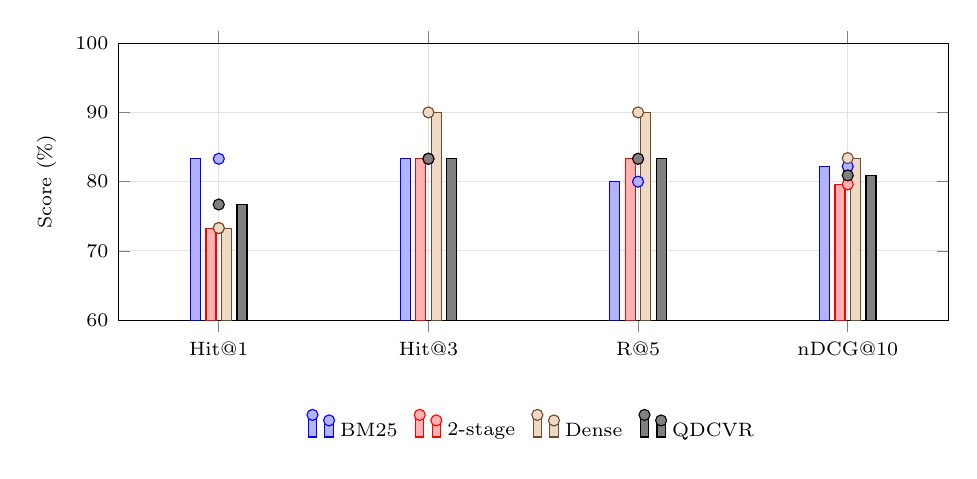
\begin{tikzpicture}
\begin{axis}[
  width=\columnwidth, height=5.1cm,
  ybar, bar width=3.6pt,
  ymin=60, ymax=100,
  ylabel={Score (\%)},
  symbolic x coords={Hit1, Hit3, R5, nDCG10},
  xtick=data,
  xticklabels={Hit@1, Hit@3, R@5, nDCG@10},
  x tick label style={font=\scriptsize},
  y tick label style={font=\scriptsize},
  ylabel style={font=\scriptsize},
  legend style={font=\scriptsize, at={(0.5,-0.30)}, anchor=north, legend columns=4,
                draw=none, /tikz/every even column/.append style={column sep=4pt}},
  enlarge x limits=0.16,
  grid=major, grid style={gray!22},
]
\addplot+[mark=*] coordinates {(Hit1,83.3) (Hit3,83.3) (R5,80.0) (nDCG10,82.2)};
\addlegendentry{BM25}
\addplot+[mark=*] coordinates {(Hit1,73.3) (Hit3,83.3) (R5,83.3) (nDCG10,79.6)};
\addlegendentry{2-stage}
\addplot+[mark=*] coordinates {(Hit1,73.3) (Hit3,90.0) (R5,90.0) (nDCG10,83.4)};
\addlegendentry{Dense}
\addplot+[mark=*] coordinates {(Hit1,76.7) (Hit3,83.3) (R5,83.3) (nDCG10,80.9)};
\addlegendentry{QDCVR}
\end{axis}
\end{tikzpicture}
\caption{BEIR SciFact (30 official queries, official qrels). Dense retrieval keeps a
small top-rank edge; QDCVR recovers Hit@1 while matching on recall. Absolute gaps are
within a few points --- see \S\ref{sec:honest} for the honest reading.}
\label{fig:scifact}
\end{figure}
